\chapter{Apparatus characterisation and test procedure}
\label{ch:characterisation}%
% Aim: 15-20 pages. This is an original contribution of the thesis: how the measured oil pressure and
% displacement are turned into stress and strain on the sample, and with what uncertainty.

The compaction vessel measures three quantities: the oil pressure $p$, the volume of oil $V$ delivered by the controller and the reading $x$ of the external LVDT. What is needed are the axial stress on the sample and its height as functions of time. Between the two there are several sources of error: the friction of the piston seals, the compliance of the oil circuit, the limited range of the LVDT, leaks, temperature changes of the oil in the line and the friction between the sample and the chamber wall. This chapter quantifies each of them, using a test without a sample and the first compaction tests, and derives the test procedure, the data reduction and the uncertainty budget used in the rest of the thesis.

The tests used for the characterisation are listed in Table~\ref{tab:commissioning}. They were carried out in the first weeks of the campaign, while the procedure was being developed. Their compaction results are reported in Appendix~\ref{app:tests}; here they serve only to characterise the apparatus.

\begin{table}[H]
    \centering
    \caption{Tests used to characterise the apparatus.}
    \label{tab:commissioning}
    \begin{tabularx}{\textwidth}{|l|>{\raggedright\arraybackslash}p{4.2cm}|>{\raggedright\arraybackslash}X|}
        \hline
        \textbf{Test} & \textbf{Sample and conditions} & \textbf{Used for} \\
        \hline
        F199 & no sample; volume control, 4.9\,cm$^3$ in 10\,min & seal friction; LVDT against oil volume \\
        \hline
        F202 & first loading trials & behaviour of the controller in volume control and with pressure limits \\
        \hline
        F203 & 18\,g of granular ice, $-10\,^\circ$C, target 3\,MPa, 1.5\,h & compliance on unloading; oil-volume displacement checked against measured heights \\
        \hline
        F204 & 12.25\,g ice + 12.25\,g quartz sand, $-20\,^\circ$C, 2\,MPa, 41\,h with unload--reload & seal friction during the step load; LVDT range; compliance; leak; thermal drift \\
        \hline
    \end{tabularx}
\end{table}

% ---------------------------------------------------------------------------
\section{Piston seal friction}
\label{sec:seal_friction}
% ---------------------------------------------------------------------------

\subsection{Measurement without a sample}

The O-rings that seal the oil chamber around the piston (Figure~\ref{fig:vessel}) resist the motion of the piston. With no sample in the chamber, the piston moves as soon as the oil pressure overcomes this friction, and the oil pressure recorded while the piston moves is a direct measurement of the seal friction expressed as a stress, $\sigma_{\mathrm{seal}}$. The same approach was used to calibrate the seal friction of the vessel for the firn compaction experiments~\cite{firn_inprep}.

In test F199 the piston, previously pushed back into its housing, was driven into the empty chamber in volume control, by pumping 4.9\,cm$^3$ of oil in about 10 minutes. The piston moved by 9.25\,mm at an average velocity of about 15\,$\mu$m/s. Figure~\ref{fig:seal_friction} shows the oil pressure as a function of the piston displacement measured by the LVDT. Three features are evident:
\begin{itemize}
    \item \textbf{a breakaway peak} of 1330\,kPa at the very start (0.23\,mm of displacement): this is the static friction of seals that have been at rest, after the piston was struck back into place;
    \item \textbf{a transition} over the first 1.7\,mm, during which the pressure falls from about 1000\,kPa to the sliding level;
    \item \textbf{a sliding level} with a mean of 420\,kPa, varying between 340 and 570\,kPa with the position of the piston, with a broad local maximum at about 5.4\,mm.
\end{itemize}

\begin{figure}[H]
    \centering
    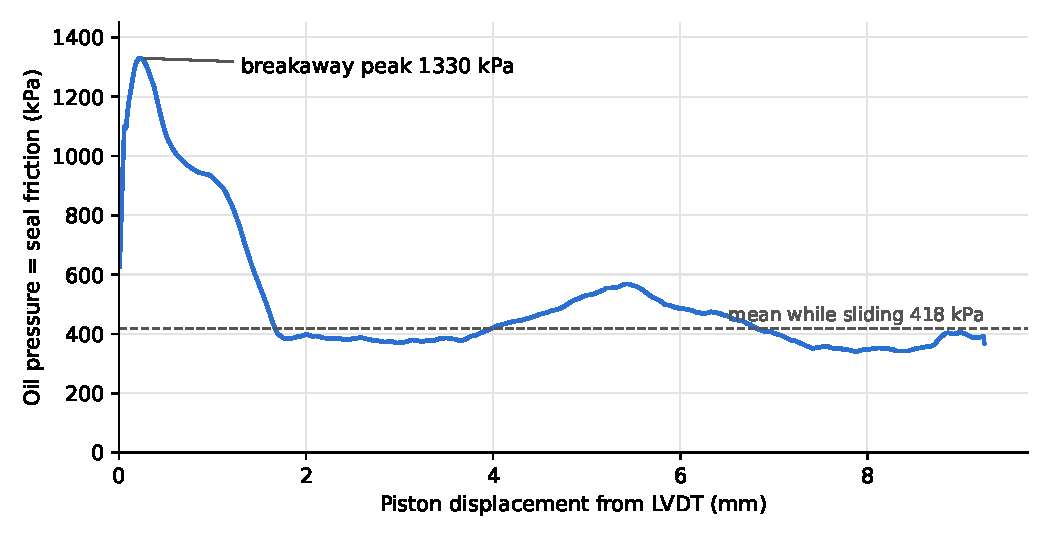
\includegraphics[width=0.85\textwidth]{Images/fig_seal_friction.pdf}
    \caption{Oil pressure against piston displacement in the test without a sample (F199, volume control, about 15\,$\mu$m/s). The pressure equals the seal friction.}
    \label{fig:seal_friction}
\end{figure}

\subsection{Measurement during a test}

The seal friction can also be read during the step load of each compaction test. When the valve to the vessel is opened, the line, pressurised to the target, discharges into the oil chamber and the piston moves quickly towards the sample, through the gap above the upper frit and into the loose sample. While the piston runs with little resistance from the sample, the pressure drops to the level needed to overcome the seals, and stays there until the sample starts to resist. In F204 (Figure~\ref{fig:start}a) this level was $215\pm8$\,kPa between 2 and 7\,s after opening, at a piston velocity of about 1.8\,mm/s. In F203 it was about 220\,kPa.

The in-test value is lower than the sliding level measured in F199. Two effects contribute. The piston is at a different position in its housing in each test, and F199 showed that the friction changes with position. The velocity differs by two orders of magnitude, and elastomer seals generally show lower friction at higher sliding velocities. Moreover, the pressure is measured at the controller, so during fast flow it slightly overestimates the pressure in the oil chamber, which would make the true in-test friction even lower.

\subsection{Consequences for the applied stress}

The axial stress applied by the piston to the top of the sample is
\begin{equation}
    \sigma_a = p - \sigma_{\mathrm{seal}},
    \label{eq:sigma_a}
\end{equation}
where $\sigma_{\mathrm{seal}}$ is the friction that acts against the motion of the piston. During a compaction test the piston never stops, since the sample keeps creeping, so the relevant value is the sliding friction at the very low velocities of the creep stage (about 1\,$\mu$m/s after 15\,min and 0.1\,$\mu$m/s after 2\,h in F204). It has not been measured directly at these velocities.
% TODO: run the empty-vessel test at 2-3 flow rates spanning 0.1-100 um/s and over the full stroke used in the tests, as in the firn calibration.
In the firn compaction experiments, empty-vessel tests at velocities from about 0.1 to 100\,$\mu$m/s gave a seal friction that depended on the piston displacement but little on velocity, except at the slowest velocity for displacements above about 12\,mm~\cite{firn_inprep}.

In this thesis $\sigma_{\mathrm{seal}}$ is taken, for each test, as the plateau of pressure measured during the step load, and the range 210--420\,kPa found above is used to estimate its uncertainty (Section~\ref{sec:uncertainty}). Two consequences follow.
\begin{itemize}
    \item \textbf{Minimum target pressure.} An uncertainty of about $\pm100$\,kPa on $\sigma_{\mathrm{seal}}$ is $\pm5\%$ of the applied stress at a target of 2\,MPa, but $\pm25\%$ at 0.5\,MPa. Targets below about 1\,MPa are therefore affected by a large uncertainty, unless the seal friction is calibrated as a function of position and velocity.
    \item \textbf{Static friction on reloading.} When the piston has been at rest, it can only move again once the oil pressure exceeds the static friction, which may be close to the breakaway value of 1330\,kPa. While the piston is stationary, the stress on the sample is not known: it lies anywhere between $p - \sigma_{\mathrm{static}}$ and $p$. This matters for the interpretation of unloading--reloading stages: if the piston does not move on reloading, this may be due to the sample being stiffer, to the static friction of the seals, or both (Chapter~\ref{ch:results}).
\end{itemize}

% ---------------------------------------------------------------------------
\section{System compliance}
\label{sec:compliance}
% ---------------------------------------------------------------------------

When the pressure rises, part of the oil delivered by the controller does not move the piston: it is stored in the circuit by the compressibility of the oil and by the expansion of the tubing, fittings and chambers. The volume stored as a function of pressure, $S(p)$, must be subtracted before the oil volume is converted into displacement.

$S(p)$ was measured during the final unloading of each test. At that stage the sample has been compacted for hours under the target stress, and the piston does not move appreciably while the pressure is decreased from the target to about 10\,kPa: the volume of oil returned to the controller is the volume released by the circuit. Figure~\ref{fig:compliance} shows the curves measured in F203 and F204. They are slightly non-linear, stiffer at higher pressures:
\begin{itemize}
    \item about 0.62\,cm$^3$/MPa between 0 and 0.5\,MPa;
    \item about 0.49\,cm$^3$/MPa between 0.5 and 1\,MPa;
    \item about 0.43\,cm$^3$/MPa between 1 and 2\,MPa.
\end{itemize}
In total, about 1.0\,cm$^3$ of oil is stored at 2\,MPa and 1.45\,cm$^3$ at 3\,MPa. Through Equation~\eqref{eq:dx_volume}, 1\,cm$^3$ corresponds to 2\,mm of apparent piston travel, so the compliance correction is of the same order as the creep compaction and cannot be neglected. The two curves differ by about 5\% at 2\,MPa, a difference that can come from the different volume of oil in the chamber (different piston position) and from small amounts of trapped air.

\begin{figure}[H]
    \centering
    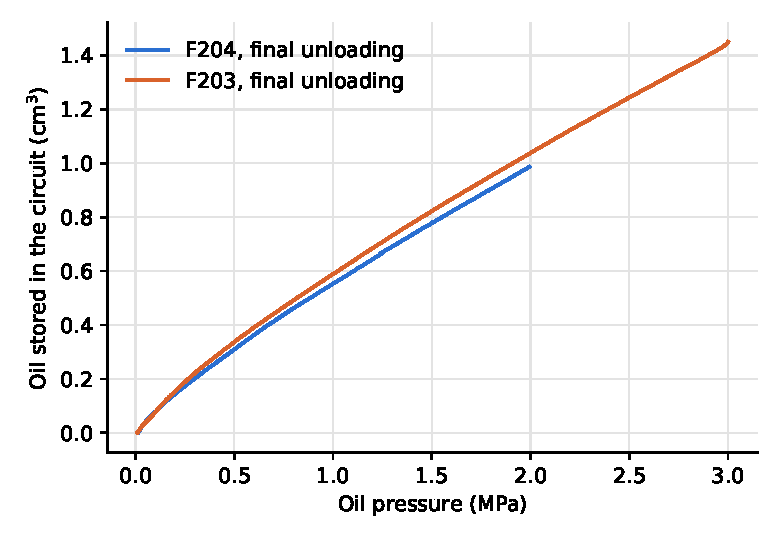
\includegraphics[width=0.62\textwidth]{Images/fig_compliance.pdf}
    \caption{Volume of oil stored in the circuit as a function of the oil pressure, measured during the final unloading of tests F203 and F204, with the piston stationary.}
    \label{fig:compliance}
\end{figure}

The unloading method assumes that the sample does not expand during unloading. Any elastic rebound of the sample pushes the piston up and returns additional oil, so the measured $S(p)$ is an upper bound of the circuit compliance. A direct measurement, independent of the sample, can be obtained by pressurising the line against the closed valve before each test, which is already part of the loading procedure (Section~\ref{sec:procedure}). This measures the compliance of the line and controller, but not that of the oil chamber in the vessel.
% TODO: record volume and pressure during the closed-valve pressurisation in every test, and compare with the unloading curve.

% ---------------------------------------------------------------------------
\section{Displacement measurement and its limits}
\label{sec:lvdt}
% ---------------------------------------------------------------------------

\subsection{Agreement between LVDT and oil volume}

In the test without a sample (F199) the pressure stayed below 600\,kPa during most of the motion, so the compliance correction was small. A linear fit of the oil volume against the LVDT displacement gave 0.505\,cm$^3$/mm, against the value of 0.507\,cm$^3$/mm expected from the piston area. The two measurements agree within 0.5\%.

At the start of F204 (Figure~\ref{fig:start}b), during the fast run of the piston into the sample, the displacement computed from the oil volume (with the compliance correction) matched the LVDT within 0.05\,mm between 3 and 10\,mm of travel. This confirms that the oil volume gives a reliable measurement of the piston displacement, including during fast events.

\begin{figure}[H]
    \centering
    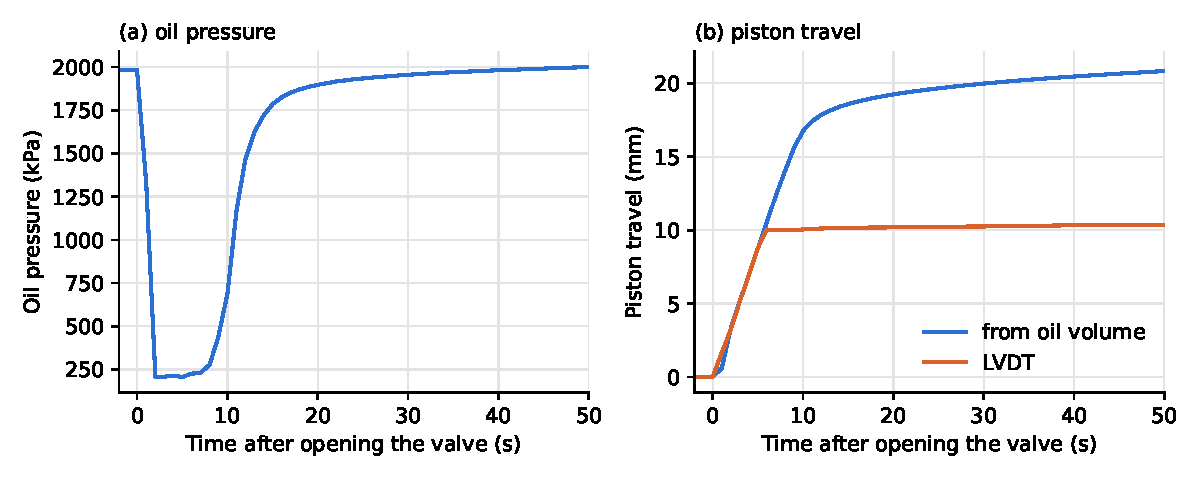
\includegraphics[width=\textwidth]{Images/fig_start.pdf}
    \caption{First 50\,s of test F204 after the valve to the vessel was opened: (a) oil pressure; (b) piston travel from the oil volume (corrected for compliance) and from the LVDT. The LVDT reached the end of its range after 10\,mm of travel.}
    \label{fig:start}
\end{figure}

\subsection{Range of the LVDT}

The LVDT is calibrated for negative readings only, and the readings close to zero are unreliable. At the other end, its reading stopped following the piston at about $-19.6$\,mm in F204, after 10\,mm of travel from the starting position of $-9.55$\,mm (Figure~\ref{fig:start}b). In F203 the reading also stayed almost constant, at about $-17.7$ to $-18.3$\,mm, while the oil volume and the measured final height showed several millimetres of further compaction. The usable interval of the LVDT is therefore from about $-6$ to about $-17$\,mm, that is, about 11\,mm.
% TODO: check the LVDT range with a caliper or gauge blocks over the whole stroke and give the calibrated interval.

The total compaction of a loose sample (about 20\,mm in F203 and F204) exceeds this interval, and most of it takes place in the first minute of the test. With the procedure used in these tests, in which the LVDT is set before loading, the LVDT runs out of range during the step load and cannot measure the creep stage, which is the part of the test where its resolution is most needed. Two remedies are possible:
\begin{enumerate}
    \item reset the LVDT after the step load: once the fast compaction is over (a few minutes after loading), the LVDT body is moved so that the reading returns to about $-6$\,mm, and the offset is recorded. The creep stage, with a compaction of a few millimetres, then falls within the usable interval;
    \item replace the LVDT with one of longer stroke (at least 30\,mm).
\end{enumerate}
In both cases, the oil volume remains the reference for the step load, and the two measurements overlap during the creep stage, which allows the oil-volume corrections to be checked.

% ---------------------------------------------------------------------------
\section{Leakage and thermal drift}
\label{sec:drift}
% ---------------------------------------------------------------------------

During a long test, the oil volume can change for two reasons unrelated to the motion of the piston: oil leaking out of the circuit, and thermal expansion or contraction of the oil in the part of the line that is at laboratory temperature. Both were observed in F204, in the stages after the main creep stage (Figure~\ref{fig:drift_leak}).

\begin{figure}[H]
    \centering
    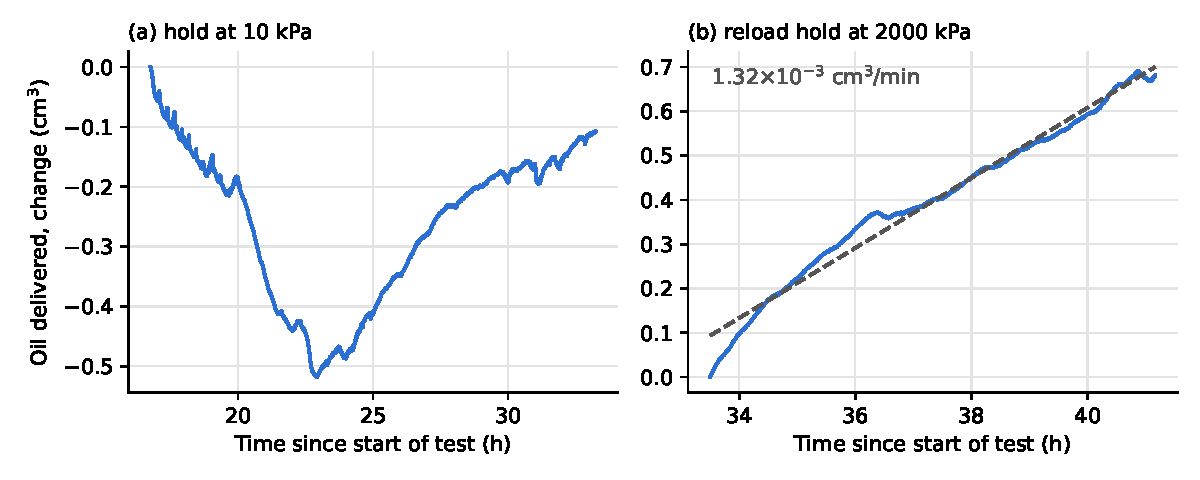
\includegraphics[width=\textwidth]{Images/fig_drift_leak.pdf}
    \caption{Oil volume during (a) the 16.6\,h hold at 10\,kPa and (b) the 7.6\,h reload hold at 2000\,kPa of test F204. In (b) the dashed line is a linear fit.}
    \label{fig:drift_leak}
\end{figure}

\paragraph{Thermal drift.} During the hold at 10\,kPa (Figure~\ref{fig:drift_leak}a), when the oil pressure is too low to cause a leak or to move the piston, the oil volume changed by about 0.5\,cm$^3$ over a day, decreasing and then increasing again with a minimum in the early afternoon. The controller keeps the pressure constant, so when the oil in the line warms up and expands, oil is withdrawn into the controller, and the opposite happens when it cools down. A day--night oscillation of $\pm0.25$\,cm$^3$ corresponds to an apparent displacement of $\pm0.5$\,mm. Part of the change in the first hours of this stage may also be due to elastic rebound of the sample after unloading; the two effects cannot be separated with the data of F204.

\paragraph{Leak.} During the reload hold at 2000\,kPa (Figure~\ref{fig:drift_leak}b) the controller delivered oil at a nearly constant rate of $1.32\times10^{-3}$\,cm$^3$/min. A constant rate over 7.6\,h is not what is expected from creep of the sample, which decelerates in time (log-linear compaction, Section~\ref{sec:firn}). It is therefore attributed to a leak, either through the piston seals or at a fitting of the line. Over the 16.6\,h of the main creep stage of F204, a leak of this size amounts to 1.3\,cm$^3$, or 2.6\,mm of apparent travel, which is about a third of the measured creep compaction. In the data reduction the leak is subtracted at a constant rate (Section~\ref{sec:data_reduction}).

Whether the leak is in the line or in the vessel can be established with a simple test: the line is pressurised to 2\,MPa against the closed valve for 2--3\,h. If the volume stays constant, the leak is in the vessel (seals); if oil is still delivered, it is in the line or the controller.
% TODO: run the leak test, find and fix the leak; report the result here.
A leak test of this kind, and a hold of a rigid dummy sample (a steel cylinder) at constant pressure, should be carried out periodically, so that the drift correction is based on a direct measurement rather than on the late stages of a compaction test.

% ---------------------------------------------------------------------------
\section{Sample--wall friction}
\label{sec:wall_friction}
% ---------------------------------------------------------------------------

As the sample is compressed, the radial stress against the chamber wall mobilises a shear stress along the wall that opposes the downward motion of the sample. Part of the axial force applied at the top is therefore carried by the wall, and the axial stress decreases with depth. This effect is well known in powder compaction and in oedometer testing. For a uniform coefficient of wall friction $\mu$ and a constant ratio $K$ between radial and axial stress, equilibrium of a slice of sample gives the classical exponential decay
\begin{equation}
    \sigma_z(z) = \sigma_a\,\exp\left(-\frac{4\,\mu K\,z}{D}\right),
    \label{eq:janssen}
\end{equation}
where $z$ is the depth below the top of the sample and $D$ its diameter. The mean axial stress over a sample of height $H$ is then
\begin{equation}
    \bar\sigma_z = \sigma_a\,\frac{1-\exp(-\beta)}{\beta}, \qquad \beta = \frac{4\,\mu K\,H}{D}.
    \label{eq:janssen_mean}
\end{equation}

The wall of the chamber is coated with a thin film of vacuum grease (Section~\ref{subsec:geometry}), which reduces $\mu$ but does not eliminate it, especially at low temperature, where the grease becomes stiffer. Neither $\mu$ nor $K$ was measured in this work: the vessel has no load cell at the bottom of the sample, so the force transmitted to the base cannot be compared with that applied at the top.

An order of magnitude can be obtained with plausible values. For granular materials in oedometric compression $K = K_0\approx0.4$--0.5, and for ice-rich materials, which behave more like a viscous fluid, $K$ approaches 1. With $\mu = 0.05$--0.10 for a greased steel wall and the height-to-diameter ratios of the tests ($H/D = 1.5$--2.4):
\begin{itemize}
    \item for $\mu K = 0.025$ (low friction), $\beta\approx0.15$--0.24, and the mean stress is 7--11\% lower than $\sigma_a$;
    \item for $\mu K = 0.10$ (high friction), $\beta\approx0.6$--1.0, and the mean stress is 25--37\% lower than $\sigma_a$.
\end{itemize}
The effect is therefore potentially larger than that of the seal friction, it acts in one direction only (it always reduces the stress), and it decreases as the sample becomes shorter during compaction. It also makes the stress non-uniform along the sample, so that the upper part densifies faster than the lower part.

Three measures limit this source of error. First, the wall is greased before every test. Second, the samples should be as short as practical: the firn experiments on the same vessel used samples about 45\,mm high ($H/D\approx1.8$), and for the mixtures of this thesis a height of 30--40\,mm ($H/D\approx1.2$--1.6) would halve $\beta$ with respect to the first tests. Third, the stresses are reported as $\sigma_a$ (the stress at the top of the sample), with the wall friction treated as a systematic error in the uncertainty budget.
% TODO: if possible, measure the density profile of a compacted sample (slices) to quantify the stress gradient.

% ---------------------------------------------------------------------------
\section{Test procedure}
\label{sec:procedure}
% ---------------------------------------------------------------------------

The procedure adopted is that of the firn compaction experiments on the same vessel, modified where the characterisation above showed it necessary. The step-by-step protocol is given in Appendix~\ref{app:protocol}; its main stages are the following.

\begin{enumerate}
    \item \textbf{Preparation of the vessel.} The chamber, piston and threads are cleaned with isopropanol; the wall is greased; the piston is pushed back into its housing with the reservoir valve open; the frits are cleaned, weighed and cooled (Section~\ref{subsec:geometry}).
    \item \textbf{Sample placement.} The sample is prepared in the cold room (Section~\ref{subsec:mixtures}) and placed in the chamber between the frits. The depth of the upper frit is measured to obtain $H_0$ (Equation~\eqref{eq:H0}), and the top cap is screwed on.
    \item \textbf{Thermal equilibration.} The sample is left in the closed vessel at the test temperature for at least one hour.
    \item \textbf{Setting the instruments.} The LVDT is set at a negative reading and its initial value recorded. The controller is programmed with the step table and with an upper pressure limit at least 400\,kPa above the target, so that the overshoot at the end of the step does not stop the test. The reservoir valve is closed, and data logging is started at 1\,Hz.
    \item \textbf{Pressurisation against the closed valve.} With the valve to the vessel closed, the controller brings the line to the target pressure. The LVDT must not move: this checks that the valve is closed and the line holds pressure.
    \item \textbf{Step load.} The valve to the vessel is opened. The piston runs into the sample, the pressure drops to the seal-friction level and then recovers to the target as the sample takes the load (Figure~\ref{fig:start}). The time of opening is recorded.
    \item \textbf{Creep stage.} The pressure is held constant for the planned duration. If the LVDT has gone out of range, it is reset to about $-6$\,mm a few minutes after loading, and the offset is recorded (Section~\ref{sec:lvdt}).
    \item \textbf{Unloading.} The pressure is reduced to about 10\,kPa with a slow ramp (30--45\,min), which gives the compliance curve $S(p)$ (Section~\ref{sec:compliance}).
    \item \textbf{End of test.} The piston protrusion is measured, the bottom of the vessel is removed and the sample is extracted. Its height and mass, and the mass of the frits, are measured immediately.
\end{enumerate}

The step load with the closed valve reproduces the procedure used for firn and makes the tests comparable with those data. Its drawback, for loose samples, is that the piston runs at high speed through the gap and into the sample, so that the first part of the compaction occurs at an unknown and varying stress. An alternative is to bring the piston into contact with the sample at a small seating stress (about 50\,kPa) before the step load, by advancing it slowly in volume control. This eliminates the gap and defines the initial state of the sample under a known stress.

\subsection{Detection of contact}

In F204 the pressure stayed at the seal-friction level for about 7\,s after the valve was opened (Figure~\ref{fig:start}a). During this time the piston travelled about 12\,mm, while the gap between piston and sample, obtained from the geometry, was only 5.8\,mm. The pressure therefore does not identify the moment of geometric contact: a loose sample is compressed by several millimetres while offering a resistance below the resolution of the pressure measurement (a few tens of kilopascals above the seal friction). The rise of the pressure above the sliding level identifies instead the moment at which the sample starts to carry a significant stress.

For this reason, the contact is defined geometrically: the gap $g$ between the lower face of the piston and the upper frit before the test is obtained from the piston length and the depth of the upper frit. The initial height $H_0$ is assigned to the sample at the moment when the piston travel equals $g$. If $g$ is not measured, it can be obtained a posteriori from the total piston travel and the measured final height (Section~\ref{sec:data_reduction}).

% ---------------------------------------------------------------------------
\section{Data reduction}
\label{sec:data_reduction}
% ---------------------------------------------------------------------------

The raw data of each test are the time series $p(t)$, $V(t)$ and $x(t)$ at 1\,Hz. They are reduced as follows.

\paragraph{Piston travel.} The piston travel since the opening of the valve, $u(t)$, is computed from the oil volume:
\begin{equation}
    u(t) = \frac{\Delta V(t) - \left[S(p(t)) - S(p_0)\right] - q\,(t-t_0)}{A},
    \label{eq:travel}
\end{equation}
where $\Delta V(t)$ is the volume delivered since the valve was opened at time $t_0$ (including the volume released by the pressurised line), $S(p)$ is the compliance curve measured at unloading, $p_0$ is the pressure just before opening, $q$ is the leak rate and $A = 0.507$\,cm$^3$/mm. Where the LVDT is within its usable range, its readings are used to check $u(t)$.

\paragraph{Sample height.} The height of the sample is
\begin{equation}
    H(t) = H_0 - \lambda\left[u(t) - g\right], \qquad u\ge g,
    \label{eq:height}
\end{equation}
where $\lambda$ is a scale factor that makes the computed final height equal to the measured one, $H_f$. For an ideal set of corrections $\lambda = 1$. In F203 the factor was 1.009, and in F204, with the leak correction, 0.94. The difference from unity measures the residual error of the corrections and is reported for every test.

\paragraph{Void ratio, density and porosity.} With the height of solids $H_s$ (Equation~\eqref{eq:e0}) and the total mass $M = m_i + m_s$:
\begin{equation}
    e(t) = \frac{H(t)}{H_s} - 1, \qquad
    \rho(t) = \frac{M}{A\,H(t)}, \qquad
    n(t) = \frac{e(t)}{1+e(t)}.
    \label{eq:state}
\end{equation}
The mass $M$ is taken from the weighed components and checked against the mass of the sample after the test. For pure ice, the relative density $D = \rho/\rho_i$ is also used, to compare with the firn literature.

\paragraph{Axial stress.} The applied axial stress is computed with Equation~\eqref{eq:sigma_a}, using the seal friction measured during the step load of the same test.

\paragraph{Time origin.} Following the firn experiments, the origin of the compaction time is set at the moment when the oil pressure first reaches 99\% of the target after the valve is opened. In F204 this occurred 40\,s after opening. The compaction before this moment is the loading stage, reported separately.

\paragraph{Strain rate.} The axial strain rate is
\begin{equation}
    \dot\varepsilon = -\frac{1}{H}\frac{\mathrm{d}H}{\mathrm{d}t}.
    \label{eq:strain_rate}
\end{equation}
Differentiating data recorded at 1\,Hz amplifies the noise. Following the firn experiments, $H(t)$ is fitted with a straight line in $\log_{10} t$ over a moving window of constant width in log-time, $[\log_{10}t - 0.1,\ \log_{10}t + 0.1]$. The derivative of the fit at the centre of the window gives $\mathrm{d}H/\mathrm{d}t$. The window therefore covers a few seconds at the start of the creep stage and several hours at its end.

\paragraph{Coefficient of secondary compression.} Where the void ratio decreases linearly with the logarithm of time, the slope gives the coefficient of secondary compression (Equation~\eqref{eq:isotache}):
\begin{equation}
    C_\alpha = -\frac{\Delta e}{\Delta\log_{10}t},
    \label{eq:calpha}
\end{equation}
fitted between 1 and 100\,min of compaction time unless stated otherwise.

% ---------------------------------------------------------------------------
\section{Uncertainty budget}
\label{sec:uncertainty}
% ---------------------------------------------------------------------------

Table~\ref{tab:uncertainty} summarises the sources of error discussed in this chapter and their effect on the main quantities, for a typical test at a target of 2\,MPa with a sample of about 60\,mm initial height.

\begin{table}[H]
    \centering
    \caption{Uncertainty budget for a typical test (target 2\,MPa, $H_0\approx60$\,mm, 16\,h of creep). Systematic errors act in one direction; random errors are given as $\pm$.}
    \label{tab:uncertainty}
    \footnotesize
    \renewcommand{\arraystretch}{1.15}
    \begin{tabularx}{\textwidth}{|>{\raggedright\arraybackslash}p{3.1cm}|>{\raggedright\arraybackslash}p{3.3cm}|>{\raggedright\arraybackslash}X|}
        \hline
        \textbf{Source} & \textbf{Size} & \textbf{Effect} \\
        \hline
        Seal friction & 210--420\,kPa & $\sigma_a$: $\pm5\%$ at 2\,MPa, $\pm25\%$ at 0.5\,MPa \\
        \hline
        Wall friction & $\mu K$ = 0.025--0.10 & mean stress 7--37\% below $\sigma_a$ (systematic) \\
        \hline
        Compliance $S(p)$ & $\pm5\%$ of 1.0\,cm$^3$ & travel $\pm0.1$\,mm; $e$: $\pm0.003$ \\
        \hline
        Leak & $\pm30\%$ of $1.3\times10^{-3}$\,cm$^3$/min & travel $\pm0.8$\,mm after 16\,h; $e$: $\pm0.02$; $C_\alpha$ at late times \\
        \hline
        Thermal drift & $\pm0.25$\,cm$^3$ (day--night) & travel $\pm0.5$\,mm; $e$: $\pm0.015$; spurious oscillations in $\dot\varepsilon$ \\
        \hline
        Initial height & $\pm0.1$\,mm & $e$: $\pm0.003$ \\
        \hline
        Grain density of LHS-1 & 2.75--2.81\,g/cm$^3$ & $H_s$: up to 1\% (equal volumes of ice and simulant); $e$: $\pm0.01$ \\
        \hline
        Mass loss & 0.5\,g of ice & $e_f$: +0.03 (systematic, checked by final weighing) \\
        \hline
        Temperature & $\pm0.05\,^\circ$C & creep rate $\pm0.6\%$ (with $Q = 60$\,kJ/mol) \\
        \hline
    \end{tabularx}
\end{table}

The uncertainties on the void ratio are absolute. They matter most at the end of the test, when the void ratio is small: an error of $\pm0.03$ is 6\% of the void ratio at $e = 0.5$ but 60\% at $e = 0.05$. The uncertainties on displacement are reduced by anchoring the computed height to the measured initial and final heights (Equation~\eqref{eq:height}): the anchoring removes the cumulative error at the end of the test, but not the error in the shape of the curve between the two ends.

The main conclusions are three. First, the stress is known to about $\pm5\%$ from the seal friction at targets of 2\,MPa and above, but the wall friction may reduce the mean stress in the sample by a larger and unknown amount; this is the largest source of uncertainty in the comparison between tests at different stresses and between the vessel and other apparatus. Second, the leak and the thermal drift control the uncertainty of the late creep stage, after about 100\,min, and must be measured and, if possible, eliminated. Third, temperature control is not a significant source of error. The improvements identified in this chapter (shorter samples, LVDT reset after loading, leak test, seal friction calibration over the stroke) are summarised in Chapter~\ref{ch:conclusions}.
